\section{Related Work}\label{sec:related-work}

\paragraph{Structure editing}
Structure editing has a long history, dating back
to the introduction of the Cornell Program Synthesizer
\cite{Cornell} in 1981.
Here we focus our attention on contemporary editors.

\setlength\intextsep{0pt}
\begin{wrapfigure}{r}{0.35\columnwidth}
  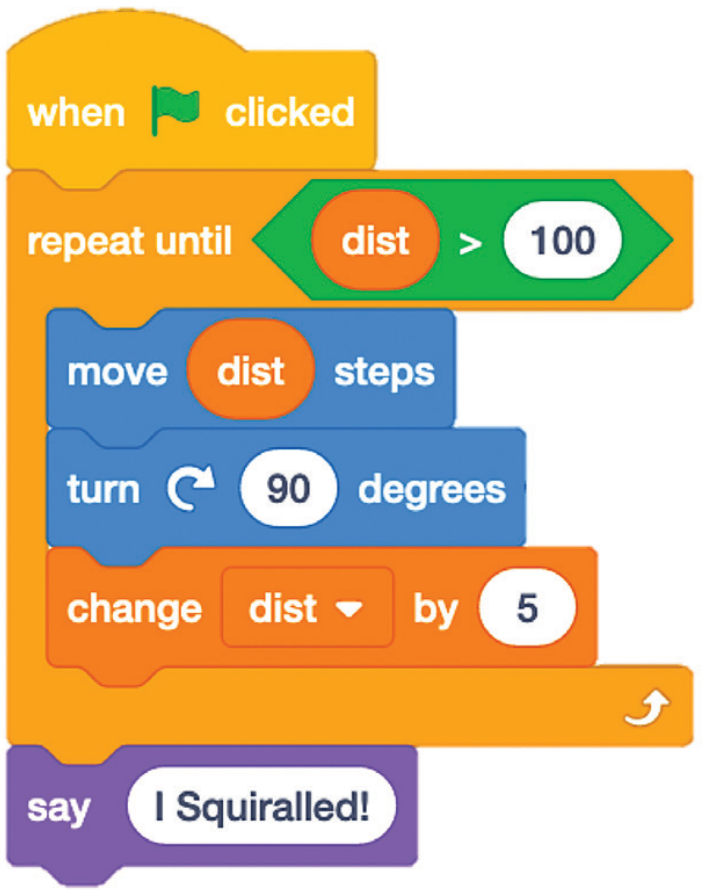
\includegraphics[width=0.4\columnwidth]{img/scratch.png}
  \caption{}
  \label{fig:scratch}
\end{wrapfigure}
The most popular structure editors today
are block-based editors such as Scratch \cite{scratch}, Snap!,
App Inventor, Alice, and many more.
In these editors, the user authors a program
like the Scratch program shown to the right
(adapted from \cite{blocks-csed})
by dragging-and-dropping blocks together on a canvas.
Each block corresponds to a syntactic form of
the underlying language and is shaped, based on its
sort, to visually indicate how it should be placed relative
to other blocks.
\tylr~ employs a similar metaphor of syntactic-forms-as-puzzle-pieces,
but uses a uniform shape system across all sorts,
thereby simplifying potential language extensions.

Block-based editors have seen great success in recent years
at introducing children to programming, but they soon
become unwieldy once users start creating and maintaining
larger or more expression-oriented programs.
For example---adapting an observation by
Brown \etal \cite{no-keyboard-cripples}---constructing
\begin{wrapfigure}{l}{0.35\columnwidth}
  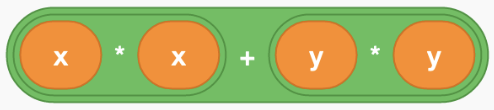
\includegraphics[width=0.4\columnwidth]{img/scratch-opseq.png}
\end{wrapfigure}
the small calculation shown on the left
involves assembling seven blocks, each
requiring a sequence of gestures to find and
drag-and-drop the appropriate block into the right spot
in the canvas;
the equivalent construction in a text editor or \tylr~ would
take seven keypresses, summing to much less effort.
% \note{need to make linear construction theme more explicit}

Meanwhile, in a user study of block-based editing
involving large refactoring tasks,
Holwerda and Hermans elicited post-task user responses
on the cognitive dimensions of block-based editing and
found that \emph{viscosity} was the most commented-on
dimension with 24 remarks.
Half (12) were positive, a majority of which
were about the ease of refactoring when the selected
elements corresponded to complete syntactic terms.
Of the negative half, half (6) were about the difficulty
of refactoring when the desired selection
does not correspond to a complete term;
for example, in Figure \ref{fig:scratch}, dragging the \code{move} block out of
the \code{repeat} block drags all the statements below
along with it, thereby requiring multiple gestures
in sum to select and remove the single \code{move} block.
These results help motivate the expressive selection
capabilities of tile-based editing.

The issue of restricted selection is not particular to
block-based editors.
Any structure editor that directly uses the
language term syntax to model
its edit state fundamentally limits selections to complete
terms.

% \note{add words + figure comparing text, structure, and tile
% editing model}

Recognizing the pitfalls of strictly term-based
editing, some structure editors
\cite{Cornell,greenfoot}
employ hybrid editing models, using structural editing
for large syntactic forms while deferring to text
editing at the leaves.
This approach loses the benefits of structure editing
at those levels, \eg, unrestricted language composition
at the expression level.
Moreover, while arbitrary text selections are possible
within a text leaf, they cannot extend beyond those
bounds and partially select any strictly structural forms.

JetBrains MPS \cite{DBLP:conf/icse/VoelterP12} is unique
among prior structure editors and similar to \tylr~ in
its aim to support keyboard-driven text-like interactions while
maintaining well-formedness at all times.
It uses an array of techniques to support text-like
editing flows, such as side tranforms to rearrange
trees in operator sequences while constructing them
linearly; and dangling parenthesis annotations in the
edit state to support constructing parentheses individually.
Despite these techniques, as a term-based editor, MPS
does not support directly selecting partial terms \cite{TowardUserFriendly}.
For example, having typed \code{2 + 3 * 4} into MPS, it would
not be possible to select \code{2 + 3} because this cuts
across the parsed associative structure.
Such a restriction is particularly pernicious in
an interface like MPS that is made to look like text, as observed
both in this example and our discussion of
difficult-to-predict deletion in Section \ref{sec:intro}.

Term-based editors as a whole can be unexpectedly
destructive when removing syntactic elements.
For example, removing a block in a block-based editor
removes all of its descendant blocks as well.
MPS mitigates this by preserving the first child of a deleted term
if they happen to share the same sort,
but cannot preserve more than one child in a generic
structure-preserving way.
Owing to its more flexible tile structure---in particular,
the convenient use of operator holes to concatenate
multiple children---\tylr~ can minimize removal
by preserving all children of the
same sort as the deleted tile.

% As with selection, term-based editors typically
% limit delete operations so they can only act on
% complete terms, which can force preemptive and tedious
% maneuvering to prevent excessive removal.
% For example, removing a block in a block-based editor
% removes all of its descendant blocks as well.
% If you intended only to delete a specific block
% while preserving its descendants, you are forced
% to save its children first by moving them elsewhere
% before you can actually delete the block.
% JetBrains MPS, a mature text-like structure editor,
% mitigates this by preserving the first child of a deleted term
% if they happen to share the same sort,
% but cannot preserve more than one child in a generic
% structure-preserving way.

% Meanwhile, it can be difficult to predict the
% effects of term-based deletion in a text-like
% interface, like MPS, that provides less visual
% indication of term structure than a block-based editor.
% Consequently a delete operation can be much
% more destructive than expected, \eg,
% pressing Backspace on a token
% causes a large containing range to disappear.
% Indeed, a (controlled) user study of MPS revealed
% that even \emph{experts} feel that deletion in MPS
% is relatively inaccurate (compared to corresponding
% subjective assessments made by text editor users),
% which we interpret to mean they have difficulty
% predicting its behavior.


% Tile-based editing reduces the destructive effect of deletions
% compared to term-based editing; moreover \tylr~ explicitly
% highlights everything that will be removed upon your deletion
% so that you never have to guess or reason through it.

% \note{discuss a bit following a text editing like flow as much
% as possible, but using restructuring to guide you in cases
% where you can't just do the text thing}

% \note{acknowledge sort-based limitations of tile structure
% in limitation section, possibly mention statements, lean into
% our philosophy but here are some thoughts}

Fructure \cite{fructure} is a structure editor for the Lisp family of
programming languages.
Similarly motivated to reduce the viscosity of structure
editing, Fructure features a novel \emph{transformation mode}
by which the user may select a term
and replace it with suggestions from an autocomplete menu.
This menu supports interactive and arbitrarily deep
construction of the replacement term before committing
the replacement; meanwhile, at each
step, the originally selected term is present in the
list of suggestions, thereby supporting expressive
wrapping of selections over the course of transformation.
The user may also ``paint'' multiple terms before
entering transformation mode, in which case the painted
terms also appear in the menu suggestions.
Fructure is strictly term-based and moreover restricted
to S-expression syntax, which has no infix operator sequences.

% Hazelnut \cite{Hazelnut} is a structure editor calculus
% similar in spirit to \ty, but with the aim of
% preserving well-typedness of its edit states.
% Hazelnut achieves this aim by developing a typed
% expression language featuring non-empty holes, which
% are automatically inserted by its type-directed action
% semantics to cordon off ill-typed portions of the program
% as they arise during editing.
% Editing in Hazelnut is strictly term-based, however, posing
% the same usability issues described earlier.
% In contrast, \ty~ and \tylr~ are untyped, the focus in
% this work being on developing more ergonomic interactions
% for maintaining syntactic well-formedness.

% \note{paragraph on structural editing plug-ins for text editors}

\paragraph{Nested words}
\ty~ segments are closely related to \emph{nested words}
\cite{nested-words},
a data representation that encodes both linear
ordering and hierarchically nested matching
of items.
A nested word consists of a sequence of letters,
some pairs of which are matching and organized
in a well nested fashion, \ie, pairs do not cross.
Segments encode a similar matching between the
constituent shards of tiles contained therein,
though \ty~ permits $n$-ary matching as opposed
to the strictly binary matching of nested words.
Nested words are well-studied from the lens of
formal language theory, but we are not aware of
any prior work that has studied editing of nested words
\ala restructuring in \tylr.

\paragraph{Zippers}
First documented by Huet
\cite{zipper}, the zipper pattern has been used to model a range of systems,
including text editors \cite{lazy-functional-incremental-parsing},
file systems \cite{zipper-fs}, and window managers \cite{window-manager}.
If the underlying structure is hierarchical,
zippers typically ask the client to navigate
in a structure-enforcing two-dimensional manner: left and right to traverse
sibling nodes, up and down to traverse parent-child relations.
In contrast, \ty~ supports a one-dimensional interaction model
in the presence of hierarchy, using disassembly to flatten
hierarchical structures as needed to support linear traversal
and partial selection.
We note that this model is distinct from using an ordered tree
traversal to linearize movement, which is still involves
strictly hierarchical navigation rather than
left-to-right navigation through a serialization of the edit state.

Some work on zippers focuses on the mechanistic \cite{derivative-zippers,clowns-jokers}
and automatic \cite{syz} generation of zipper forms
from datatypes;
these techniques are orthogonal to our tile-based zipper design
and may prove useful in future work on
automatically generating tile-based zippers
from a given syntax.

% \note{mention Parsing With Zippers}

% \paragraph{Incremental parsing}
% Zipper operations in \ty~ rely on incremental and partial
% parsing to reassemble shards as the opportunity arises.
% Existing incremental parsing techniques

% \begin{itemize}
%   \item structure editing
%   \begin{itemize}
%     \item Design Requirements for More Flexible Structured Editors from a Study of Programmers' Text Editing
%       by Amy Ko \& Brad Myers
%     \begin{itemize}
%         \item list edits (23\%):
%           removing a list element and its delimiter (8\%);
%           moving the right list delimiter(3\%);
%           ``flattening'' a list inside of a list (2\%)
%         \item infix expressions (15\%):
%             replacing the infix expression with its left (8\%) or right (1\%) operand;
%             ``wrapping'' a left or right operand (4\%);
%             unwrapping a left or right operand (2\%)
%         \item prefix expressions (1\%):
%             applying a prefix operator to an expression (81\%);
%             ``unwrapping'' a prefix operand (11\%)
%         \item that amounts to 6\% of edits clearly involving selecting and
%           moving/removing non-term selections, or 10\% of edits not involving
%           modifying names
%     \end{itemize}
%   \end{itemize}
% \end{itemize}